\documentclass[portrait,a0]{a0poster}

\usepackage[brazil]{babel}
\usepackage[T1]{fontenc}
\usepackage[utf8]{inputenc}

%\usepackage{geometry}
%\geometry{
%paperwidth=90cm,
%paperheight=120cm,
%textwidth=85cm,
%textheight=95cm,
%left=5cm,
%top=5cm
%}



\usepackage{multicol} % This is so we can have multiple columns of text side-by-side
\columnsep=30mm % This is the amount of white space between the columns in the poster
\columnseprule=3pt % This is the thickness of the black line between the columns in the poster


\usepackage[svgnames]{xcolor} % Specify colors by their 'svgnames', for a full list of all colors available see here: http://www.latextemplates.com/svgnames-colors

\usepackage{times} % Use the times font
%\usepackage{palatino} % Uncomment to use the Palatino font

\usepackage{graphicx} % Required for including images
%\usepackage{showframe}
\graphicspath{{figures/}} % Location of the graphics files
\usepackage{booktabs} % Top and bottom rules for table
\usepackage[font=small,labelfont=bf]{caption} % Required for specifying captions to tables and figures
\usepackage{amsfonts, amsmath, amsthm, amssymb} % For math fonts, symbols and environments
\usepackage{wrapfig} % Allows wrapping text around tables and figures
\usepackage{here} % Figure and table environments.
\usepackage{microtype} %Melhorias de justificação do texto.

\usepackage[
	backend = biber,
	style = abnt, % Para usar o sistema alfabético;
%	style = abnt-numeric,   % Para usar o sistema numérico;
	bftitles, %Negrito nos títulos;
	giveninits, %Abrevia primeiros nomes;
	hyperref, %Criar hyperlinks (se hyperref for usado?);
	backref %Contar quantas vezes entrada foi citada;
]{biblatex}


\addbibresource{LabFisica.bib}



\begin{document}

%----------------------------------------------------------------------------------------
%	POSTER HEADER 
%----------------------------------------------------------------------------------------

% The header is divided into two boxes:
% The first is 75% wide and houses the title, subtitle, names, university/organization and contact information
% The second is 25% wide and houses a logo for your university/organization or a photo of you
% The widths of these boxes can be easily edited to accommodate your content as you see fit

\begin{minipage}[b]{0.75\linewidth}
\renewcommand{\thefootnote}{\alph{footnote}}
\veryHuge \color{NavyBlue} \textbf{Física experimental} \color{Black}\\ % Title
\Huge\textit{Uma ferramenta de aprendizagem para engenharia}\\[2cm] % Subtitle
\huge \textbf{
Alan Cesar\footnotemark[2],
Bruno Braga\footnotemark[1],
Cristiano Coutinho\footnotemark[2],
Daniel Rebouças\footnotemark[5],
}\\[0.5cm] % Author(s)
\huge \textbf{
Davi Almeida\footnotemark[5],
Gustavo Penaforte\footnotemark[1],
Iasmin Pereira\footnotemark[3],
Raul Fontenele\footnotemark[1],
}\\[0.5cm] % Author(s)
\huge \textbf{
Ricardo Braga\footnotemark[2],
Sinara Braga\footnotemark[4],
Thiago Rabelo\footnotemark[5],
e Roberto Lima\footnotemark[6]
}\\[0.5cm] % Author(s)
\huge Universidade de Fortaleza\\[0.4cm] % University/organization
\Large \texttt{robertolima@unifor.br} \\
%
\footnotetext[1]{Estudante de Engenharia de Controle e Automação}
\footnotetext[2]{Estudante de Engenharia de Computação}
\footnotetext[3]{Estudante de Engenharia de Produção}
\footnotetext[4]{Estudante de Engenharia Mecânica}
\footnotetext[5]{Estudante de Engenharia Elétrica}
\footnotetext[6]{Professor Orientador, CCT}
\end{minipage}
%
\begin{minipage}[b]{0.25\linewidth}
%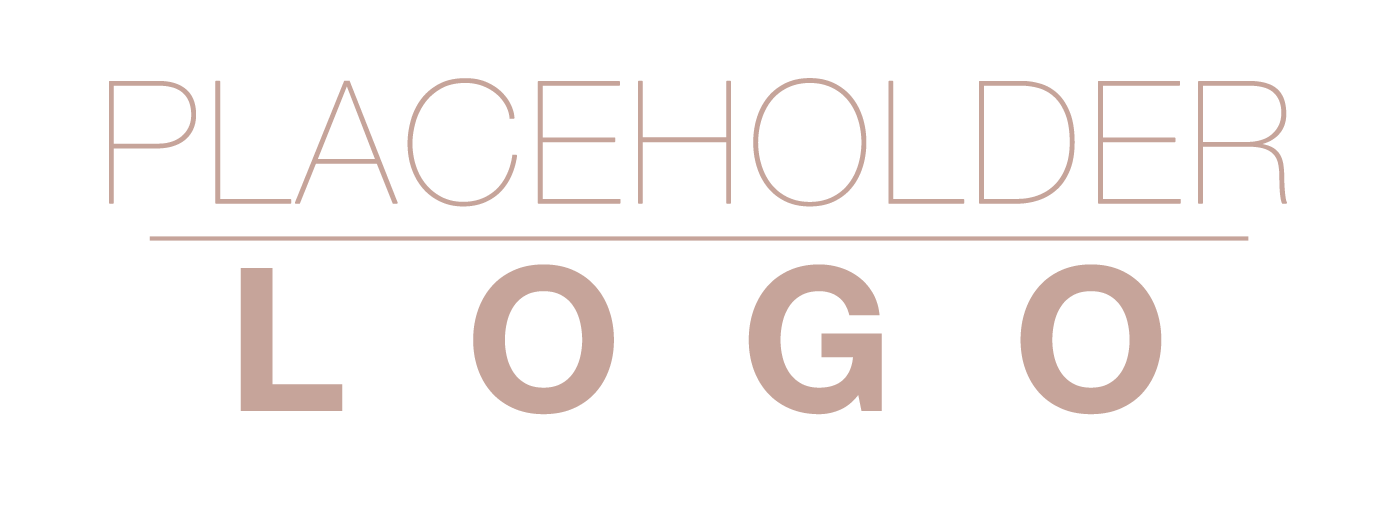
\includegraphics[width=20cm]{logo.png}\\
%
\includegraphics[width=20cm]{Unifor-logo01.pdf}\\

\includegraphics[scale=0.8]{DiaT-mod.png}\\
\end{minipage}

\vspace{1cm} % A bit of extra whitespace between the header and poster content

%----------------------------------------------------------------------------------------

\begin{multicols}{2} % This is how many columns your poster will be broken into, a portrait poster is generally split into 2 columns

%----------------------------------------------------------------------------------------
%	ABSTRACT
%----------------------------------------------------------------------------------------

%\color{Navy} % Navy color for the abstract
%
%\begin{abstract}
%Nos dias atuais as aulas convencionais em sala requerem um apoio de práticas em laboratório.
%A compreensão de alguns conteúdos pode muitas vezes ser prejudicada em vista dos alunos não terem contato direto com as situações estudadas teoricamente.
%O laboratório didático passa a ser um dispositivo importante nos estudos.
%%
%Dentro deste contexto, o presente trabalho apresenta a proposta do grupo de estudos em física experimental.
%
%\end{abstract}

%----------------------------------------------------------------------------------------
%	INTRODUCTION
%----------------------------------------------------------------------------------------

\color{SaddleBrown} % SaddleBrown color for the introduction

\section*{Introdução}

A Física é uma disciplina que muitas vezes remete à cálculos e fórmulas matemáticas.
Frequentemente é deixado de lado o teor experimental da mesma, da validade das teorias, dentro do contexto epistemológico.
Porém nos últimos anos vem se dando cada vez mais importância aos laboratórios experimentais, pois estes são apresentados como facilitadores da aprendizagem
\cite{Grandini_2004, RodriguesCunha2014}.
A motivação para aprender também é outro aspecto que deve ser ressaltado no âmbito do laboratório.
Procedimentos arcaicos podem ser uma barreira ao aprendizado, visto o atual momento tecnológico.
Muitos dispositivos de baixo custo estão disponíveis no mercado, os quais desempenham papel importante da automatização de tarefas.
Talvez o exemplo mais evidente seja a plataforma aberta \emph{Arduino}, cuja acessibilidade e facilidade de uso são os pontos chaves deste dispositivo~\cite{OliveiraZanetti2015}.
Não são necessário conhecimentos profundos sobre circuitos para se construir um projeto cheio de elementos eletrônicos que outrora apenas peritos podiam desenvolver.
Fóruns online e uma ampla documentação disponível tornam o aprendizado desta plataforma extremamente viável para qualquer pessoa com acesso à internet.


%Segundo \textcite{OliveiraZanetti2015}:
%\begin{quote}
%``O Arduino é uma plataforma de hardware open source, projetada sobre o microcontrolador Atmel AVR, que pode ser programado através de uma linguagem de programação similar a C/C++, permitindo a elaboração de projetos com um conhecimento mínimo ou mesmo nenhum de eletrônica.
%Foi criado com o objetivo de fornecer uma plataforma de fácil prototipação de projetos interativos, unindo software e hardware, características da Computação Física.''
%\end{quote}


A utilização de plataformas que envolvem programação computacional por parte do estudante podem causar um impacto positivo na aprendizagem de forma geral.
Os algoritmos computacionais estão intimamente ligados ao desenvolvimento de estruturas do raciocínio lógico, influenciando até no comportamento humano frente à tomada de decisões em problemas do cotidiano~\cite{Zanetti_2015}.
Além disso, o contato do aluno com o equipamento de modo que o mesmo possa entender seu funcionamento é tanto motivador quanto desmistificador das atividades experimentais \cite{Rosa2003}.


%----------------------------------------------------------------------------------------
%	OBJECTIVES
%----------------------------------------------------------------------------------------

\color{DarkSlateGray} % DarkSlateGray color for the rest of the content

\section*{Principais Objetivos}

\begin{enumerate}
\item Revisar os roteiros de práticas dos laboratórios de Física.
\item Estudar a Física aplicada nos procedimentos de laboratório.
\item Contextualizar as aplicações de engenharia dentro do laboratório de física.
\item Escrever textos usando a ferramenta \LaTeX.
\item Adaptar experimentos usando a plataforma \emph{Arduino}.
\end{enumerate}

%----------------------------------------------------------------------------------------
%	MATERIALS AND METHODS
%----------------------------------------------------------------------------------------

\section*{Materiais e Métodos}

Para a realização deste trabalho, reuniões semanais são realizadas no laboratório didático de Física, visando executar algumas atividades práticas bem como revisar o roteiro de prática do laboratório.
Os aparatos de laboratório também ficam à disposição, sendo que os mesmos são previamente solicitados aos técnicos de laboratório bem com aos professor orientador.
Nesta etapa inicial, a maior atenção está sendo dada à aprendizagem da ferramenta \LaTeX, assim como à revisão bibliográfica dos assuntos relacionados aos experimentos, assim como à busca de contexto que interligue de maneira mais próxima a Física à Engenharia.
O computador pessoal de cada estudante também é uma ferramenta essencial ao andamento deste projeto.


%----------------------------------------------------------------------------------------
%	RESULTS 
%----------------------------------------------------------------------------------------

\section*{Resultados}

Até o presente momento, selecionamos três experimentos para serem analisados: lançamento horizontal, propriedades ópticas e porosidade de materiais.
Embora existam os roteiros de práticas dos experimentos, alguns estão passando por revisão.
%
\begin{wraptable}{l}{12cm} % Left or right alignment is specified in the first bracket, the width of the table is in the second
\begin{tabular}{l l l}
\toprule
\textbf{Experimento} & \textbf{Intergantes} & \textbf{Roteiro}\\
\midrule
Lançamento & 5 & Completo\\
Óptica & 4 & Parcial \\
Porosidade & 4 & Parcial \\
\bottomrule
\end{tabular}
\captionof{table}{\color{Green} Práticas trabalhadas.}
\end{wraptable}
%
No experimento de lançamento horizontal, embora bastante simples, necessita de uma melhoria em relação à precisão dos dados.
Um trabalho inicial foi desenvolvido pelo estudante \emph{Raul Fontenele}, o qual apresentou e publicou o trabalho no evento \emph{Encontros Científicos} da Universidade de Fortaleza, neste ano (2016).
O trabalho está sendo aprimorado pelo grupo de estudos, assim como o roteiro da prática, o qual ainda não havia sido revisado à um certo tempo.


%\begin{center}\vspace{1cm}
%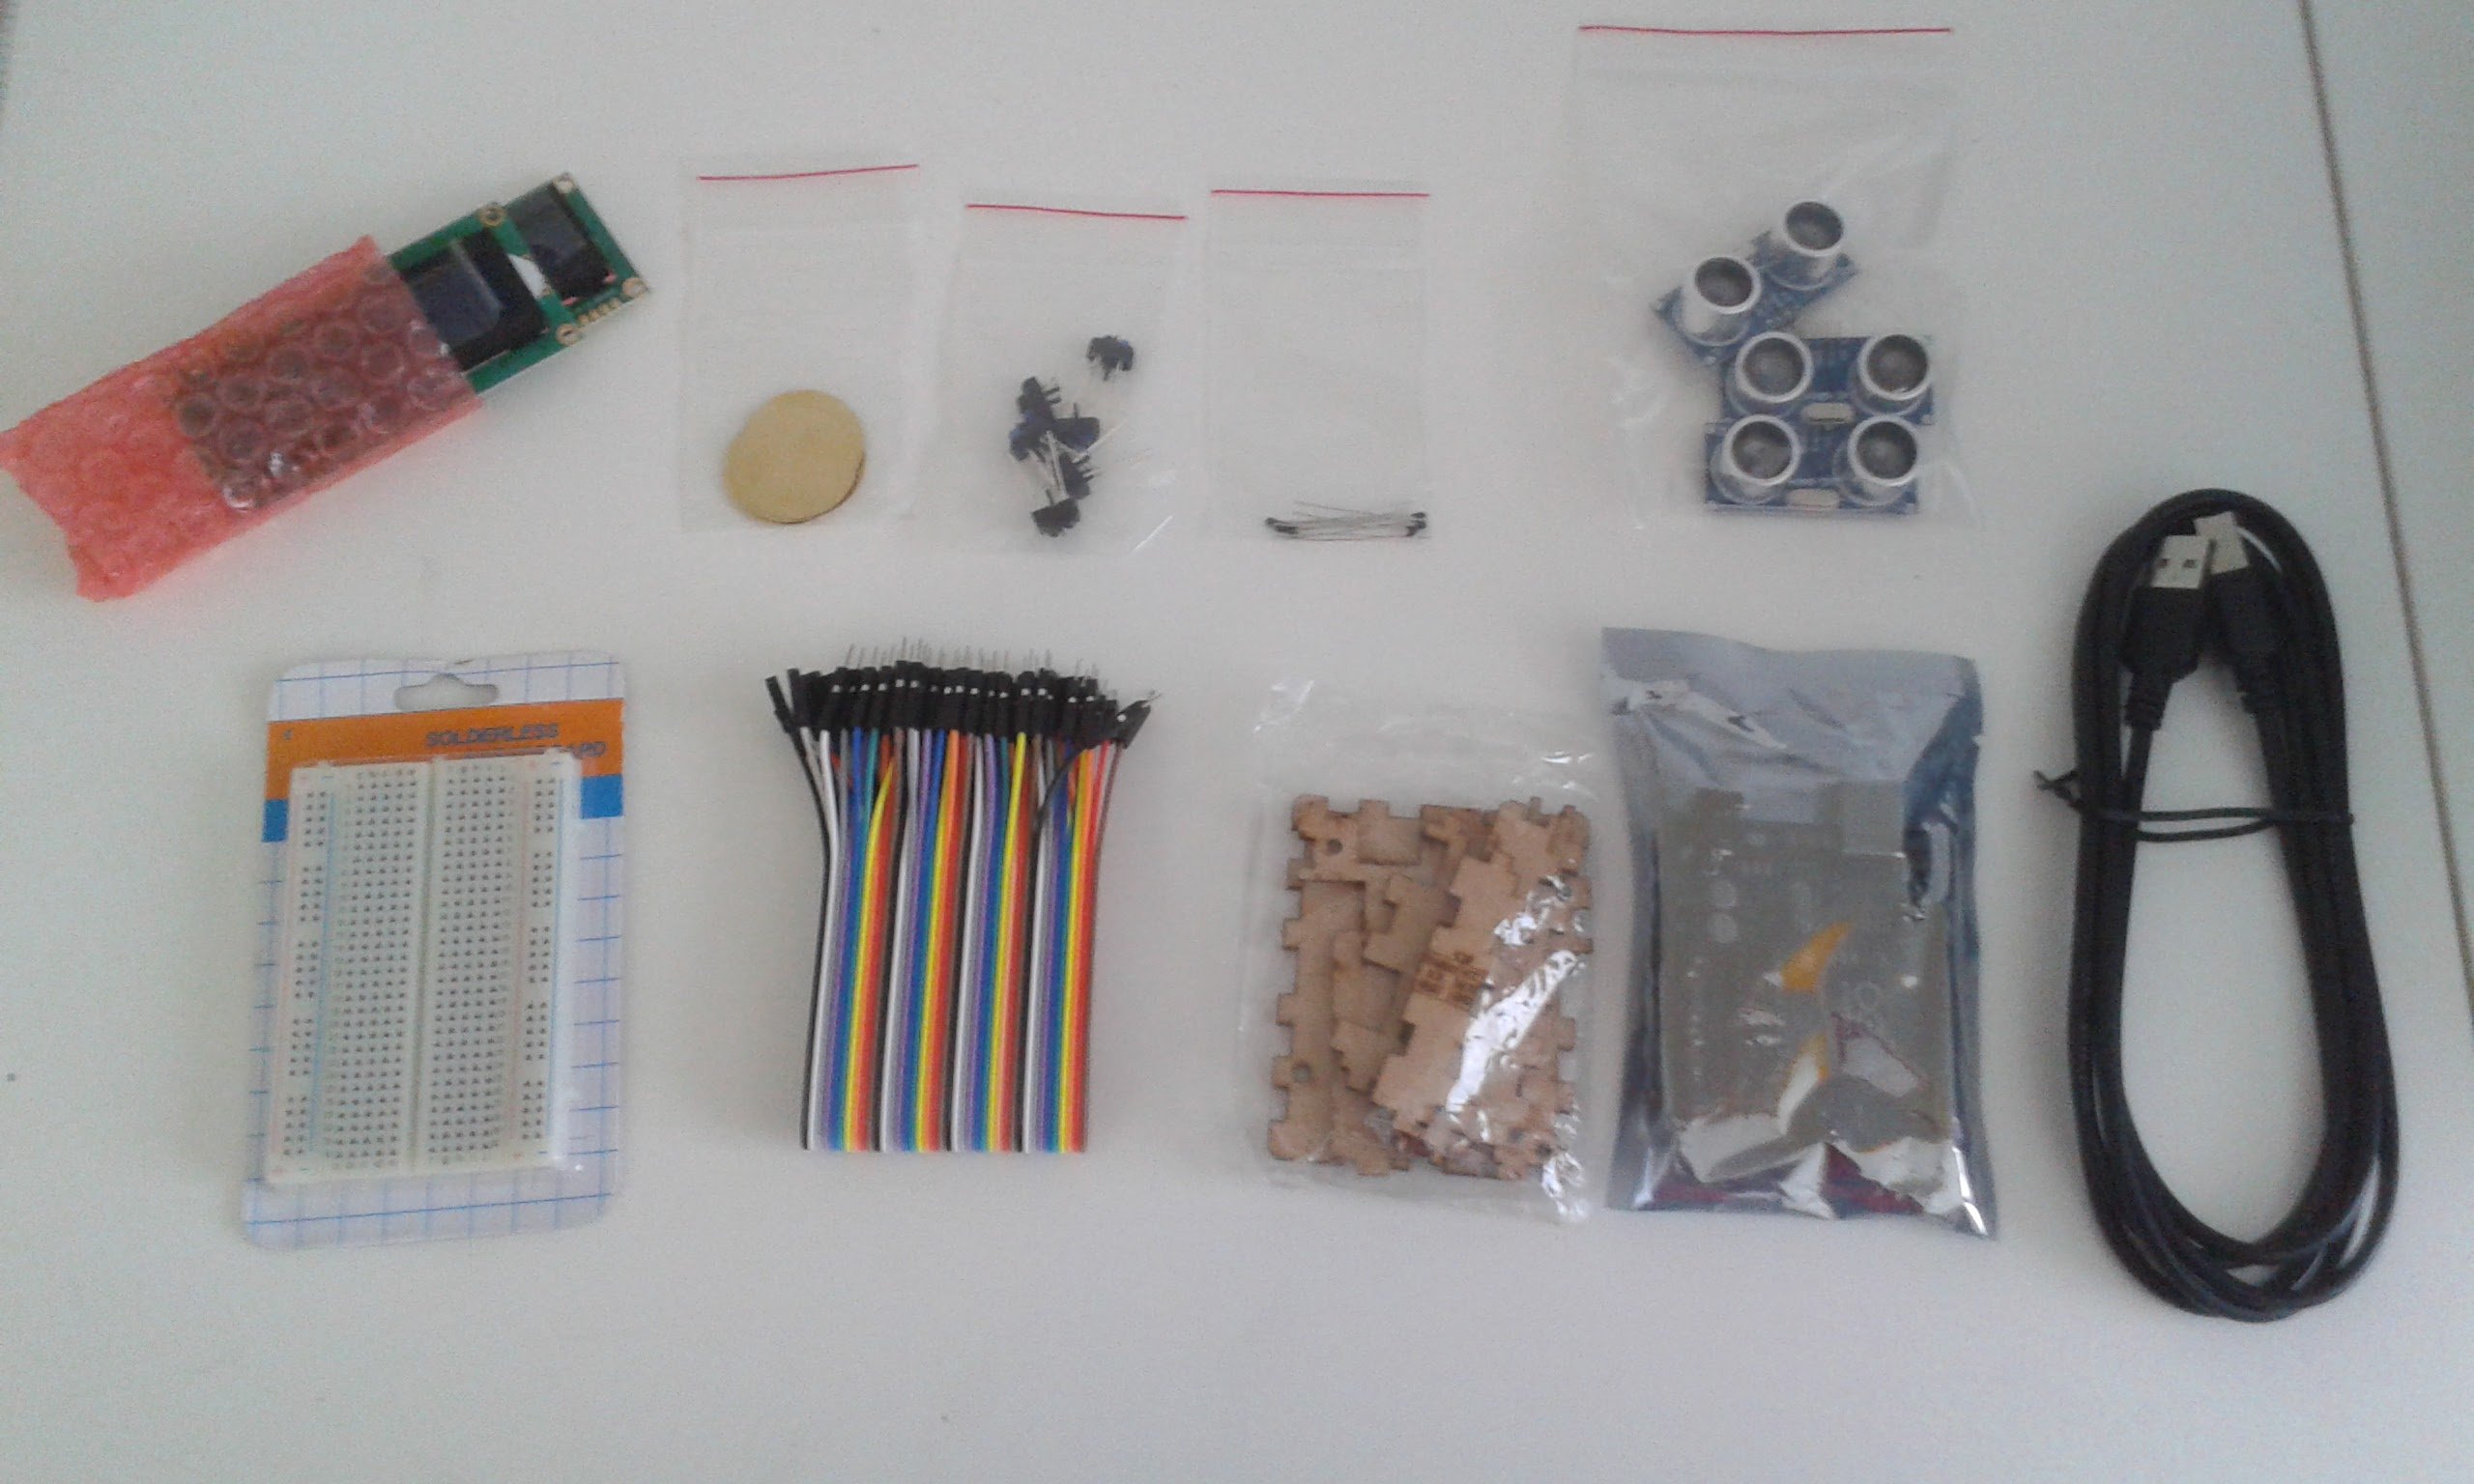
\includegraphics[scale=0.29]{materiais.jpg}
%\captionof{figure}{\color{Green} Materiais utilizados para aplicação com Arduino.}
%\end{center}\vspace{1cm}


Outros dois experimento que, embora não sejam utilizados nas práticas de disciplinas de Física atuais, são abordadas em disciplinas correlatas que usam o laboratório de Física e ministrada por professores de Física.

O primeiro é um experimento de propriedade ópticas dos materiais, que visa obter o índice de refração de um sólido transparente.
Com tal parâmetro obtido, projetos de engenharia podem ser executados para melhorar, por exemplo, a luminosidade de um certo ambiente, assim como sua eficiência.

Outro experimento que está sendo trabalhado é sobre porosidade.
Embora seja um assunto associado aos materiais, possui uma íntima ligação com a Física da difusão.
Muitos materiais modernos também usam parâmetros de porosidade em seus estudos.
Assim, o experimento já existente no laboratório está passando por uma revisão e adequação também ao projeto de ensino de algumas disciplinas.
Vale ressaltar que este é um trabalho prévio, de análise, sob orientação de um professor de Física.

\begin{table}[H]
\centering
\begin{tabular}{l l l l}
\toprule
\textbf{Experimento} & \textbf{Roteiro} & \textbf{Aparato} \\
\midrule
Momento de inércia & Completo & Disponível \\
Magnetismo da matéria & Ausente & Indisponível \\
Radiação térmica & Parcial & Incompleto \\
\bottomrule
\end{tabular}
\caption{Experimentos a serem analisados.}
\label{tab:experimentos-futuros}
\end{table}

Outros experimentos também estão sendo selecionados para futuros estudos, como os dispostos na Tabela~\ref{tab:experimentos-futuros}.

%\begin{center}\vspace{1cm}
%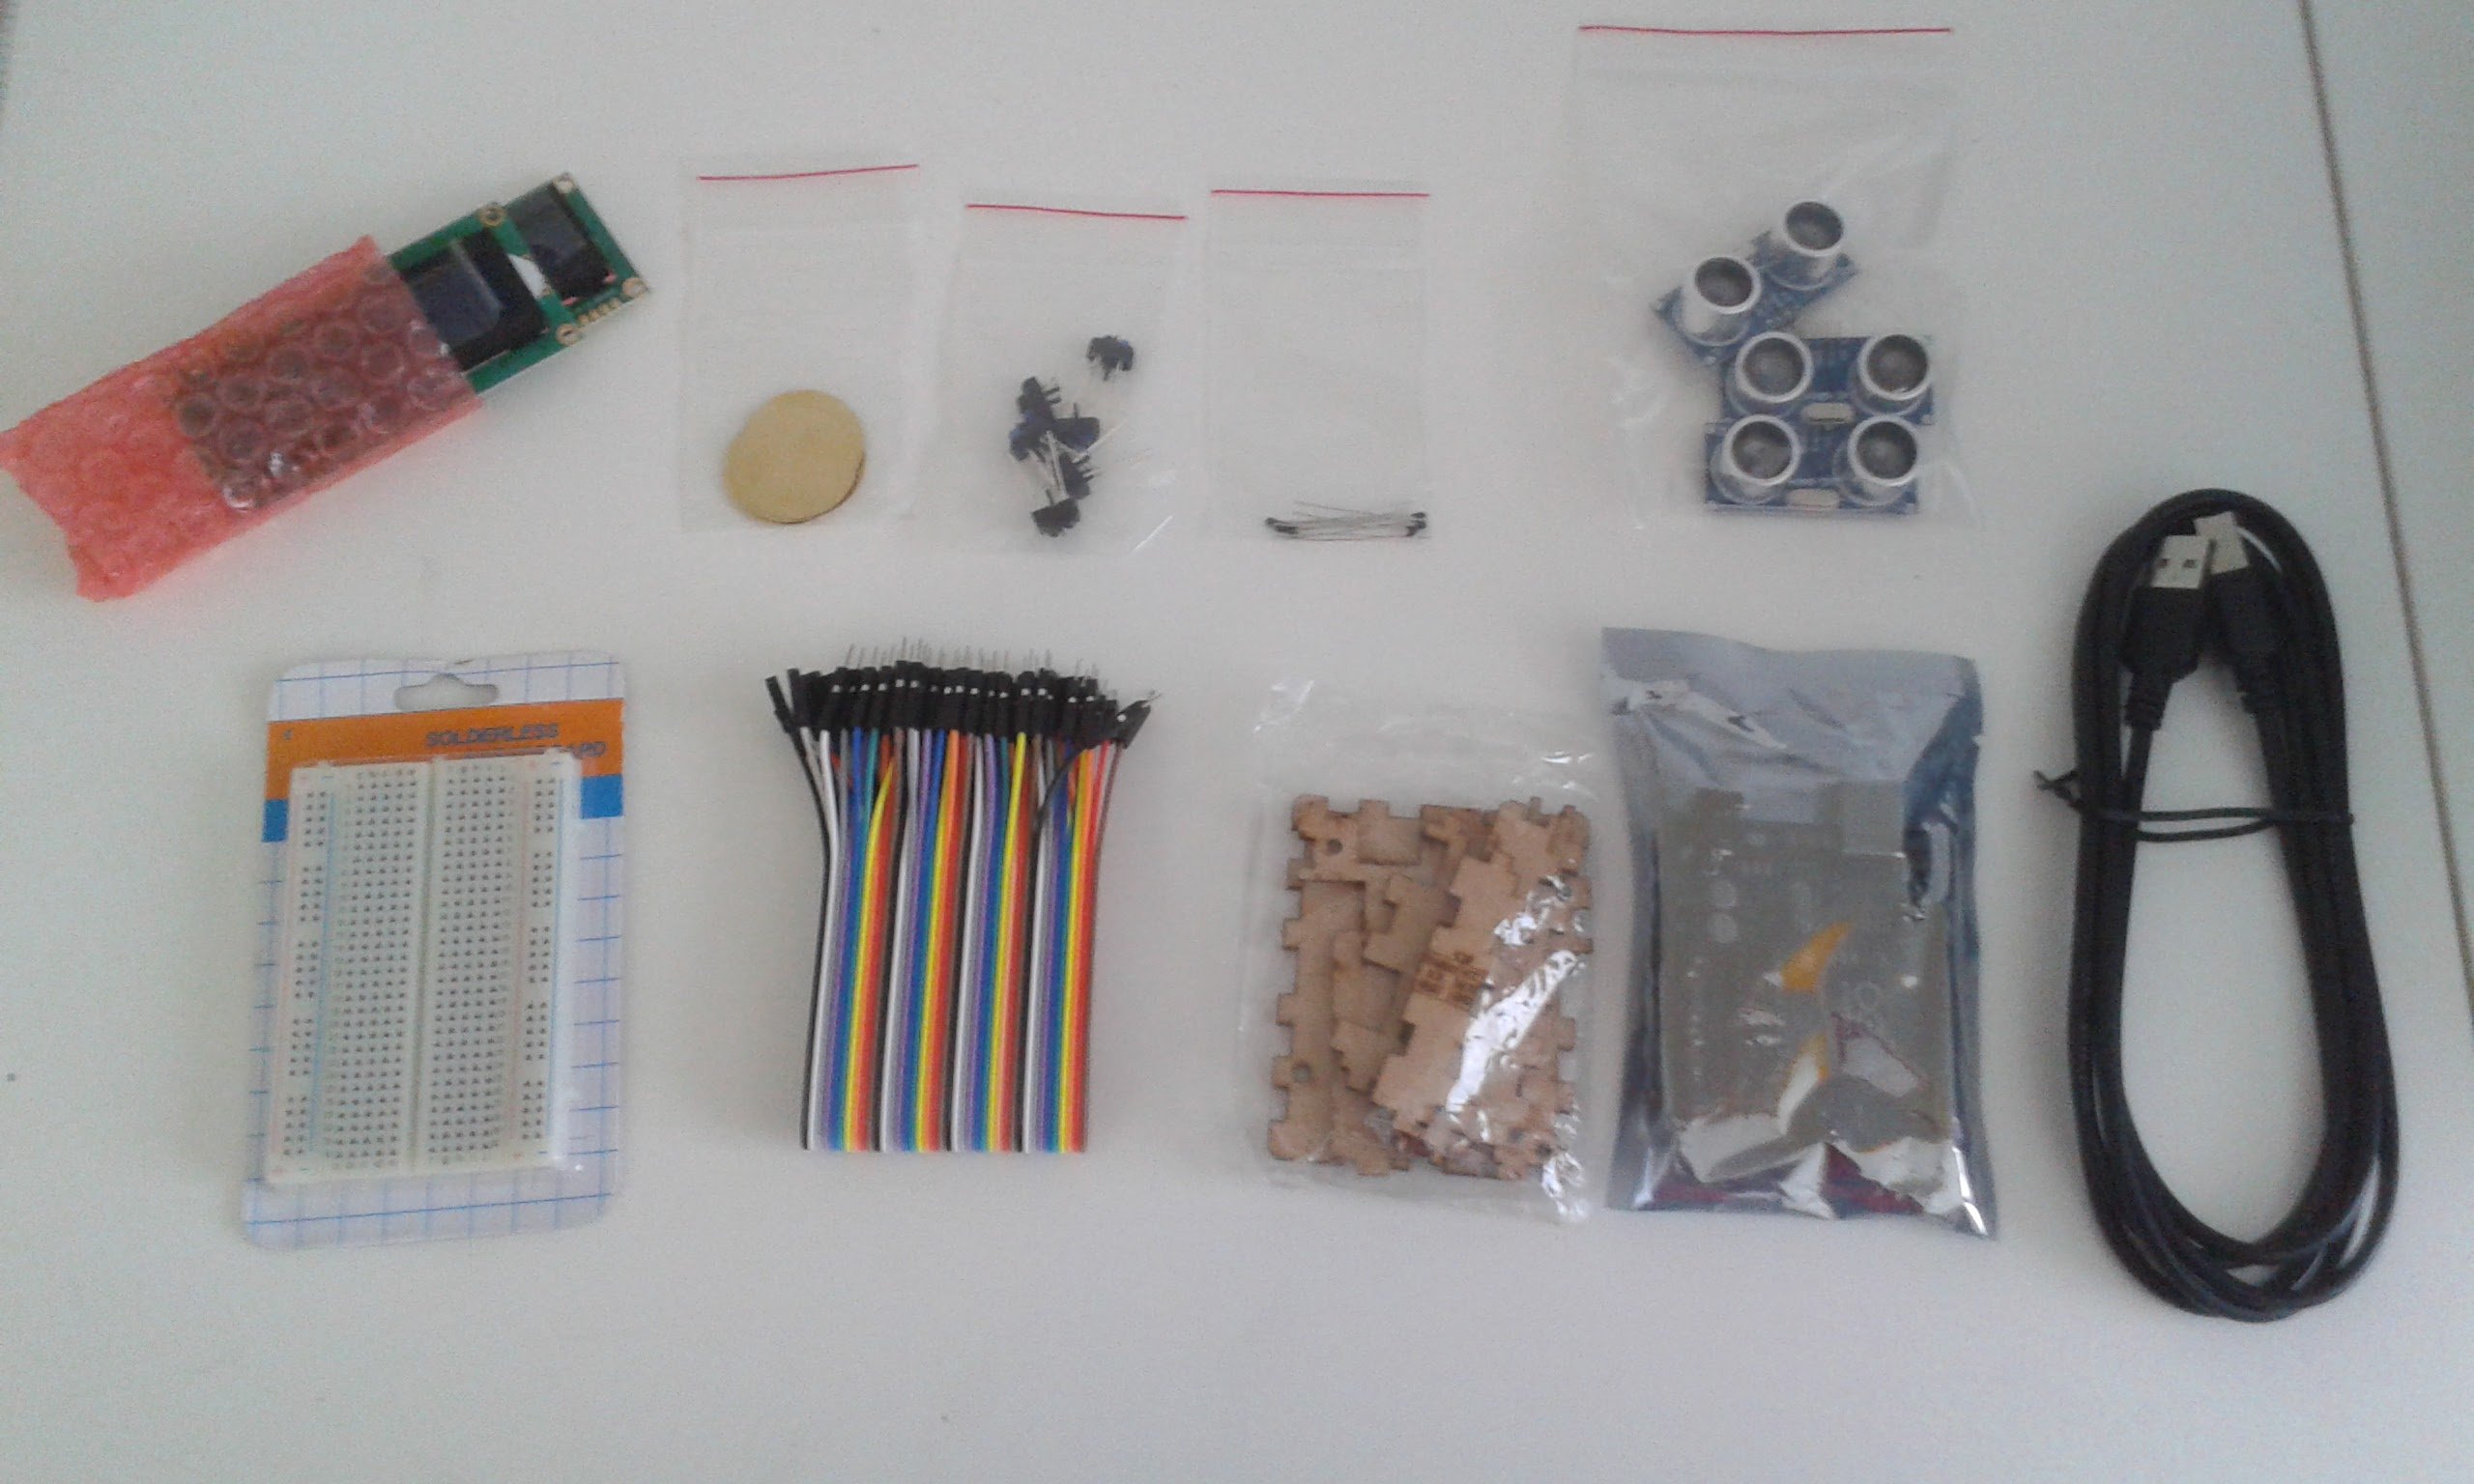
\includegraphics[width=0.8\linewidth]{materiais.jpg}
%\captionof{figure}{\color{Green} Materiais utilizados para aplicação com Arduino.}
%\end{center}\vspace{1cm}

\begin{figure}[H]
\centering
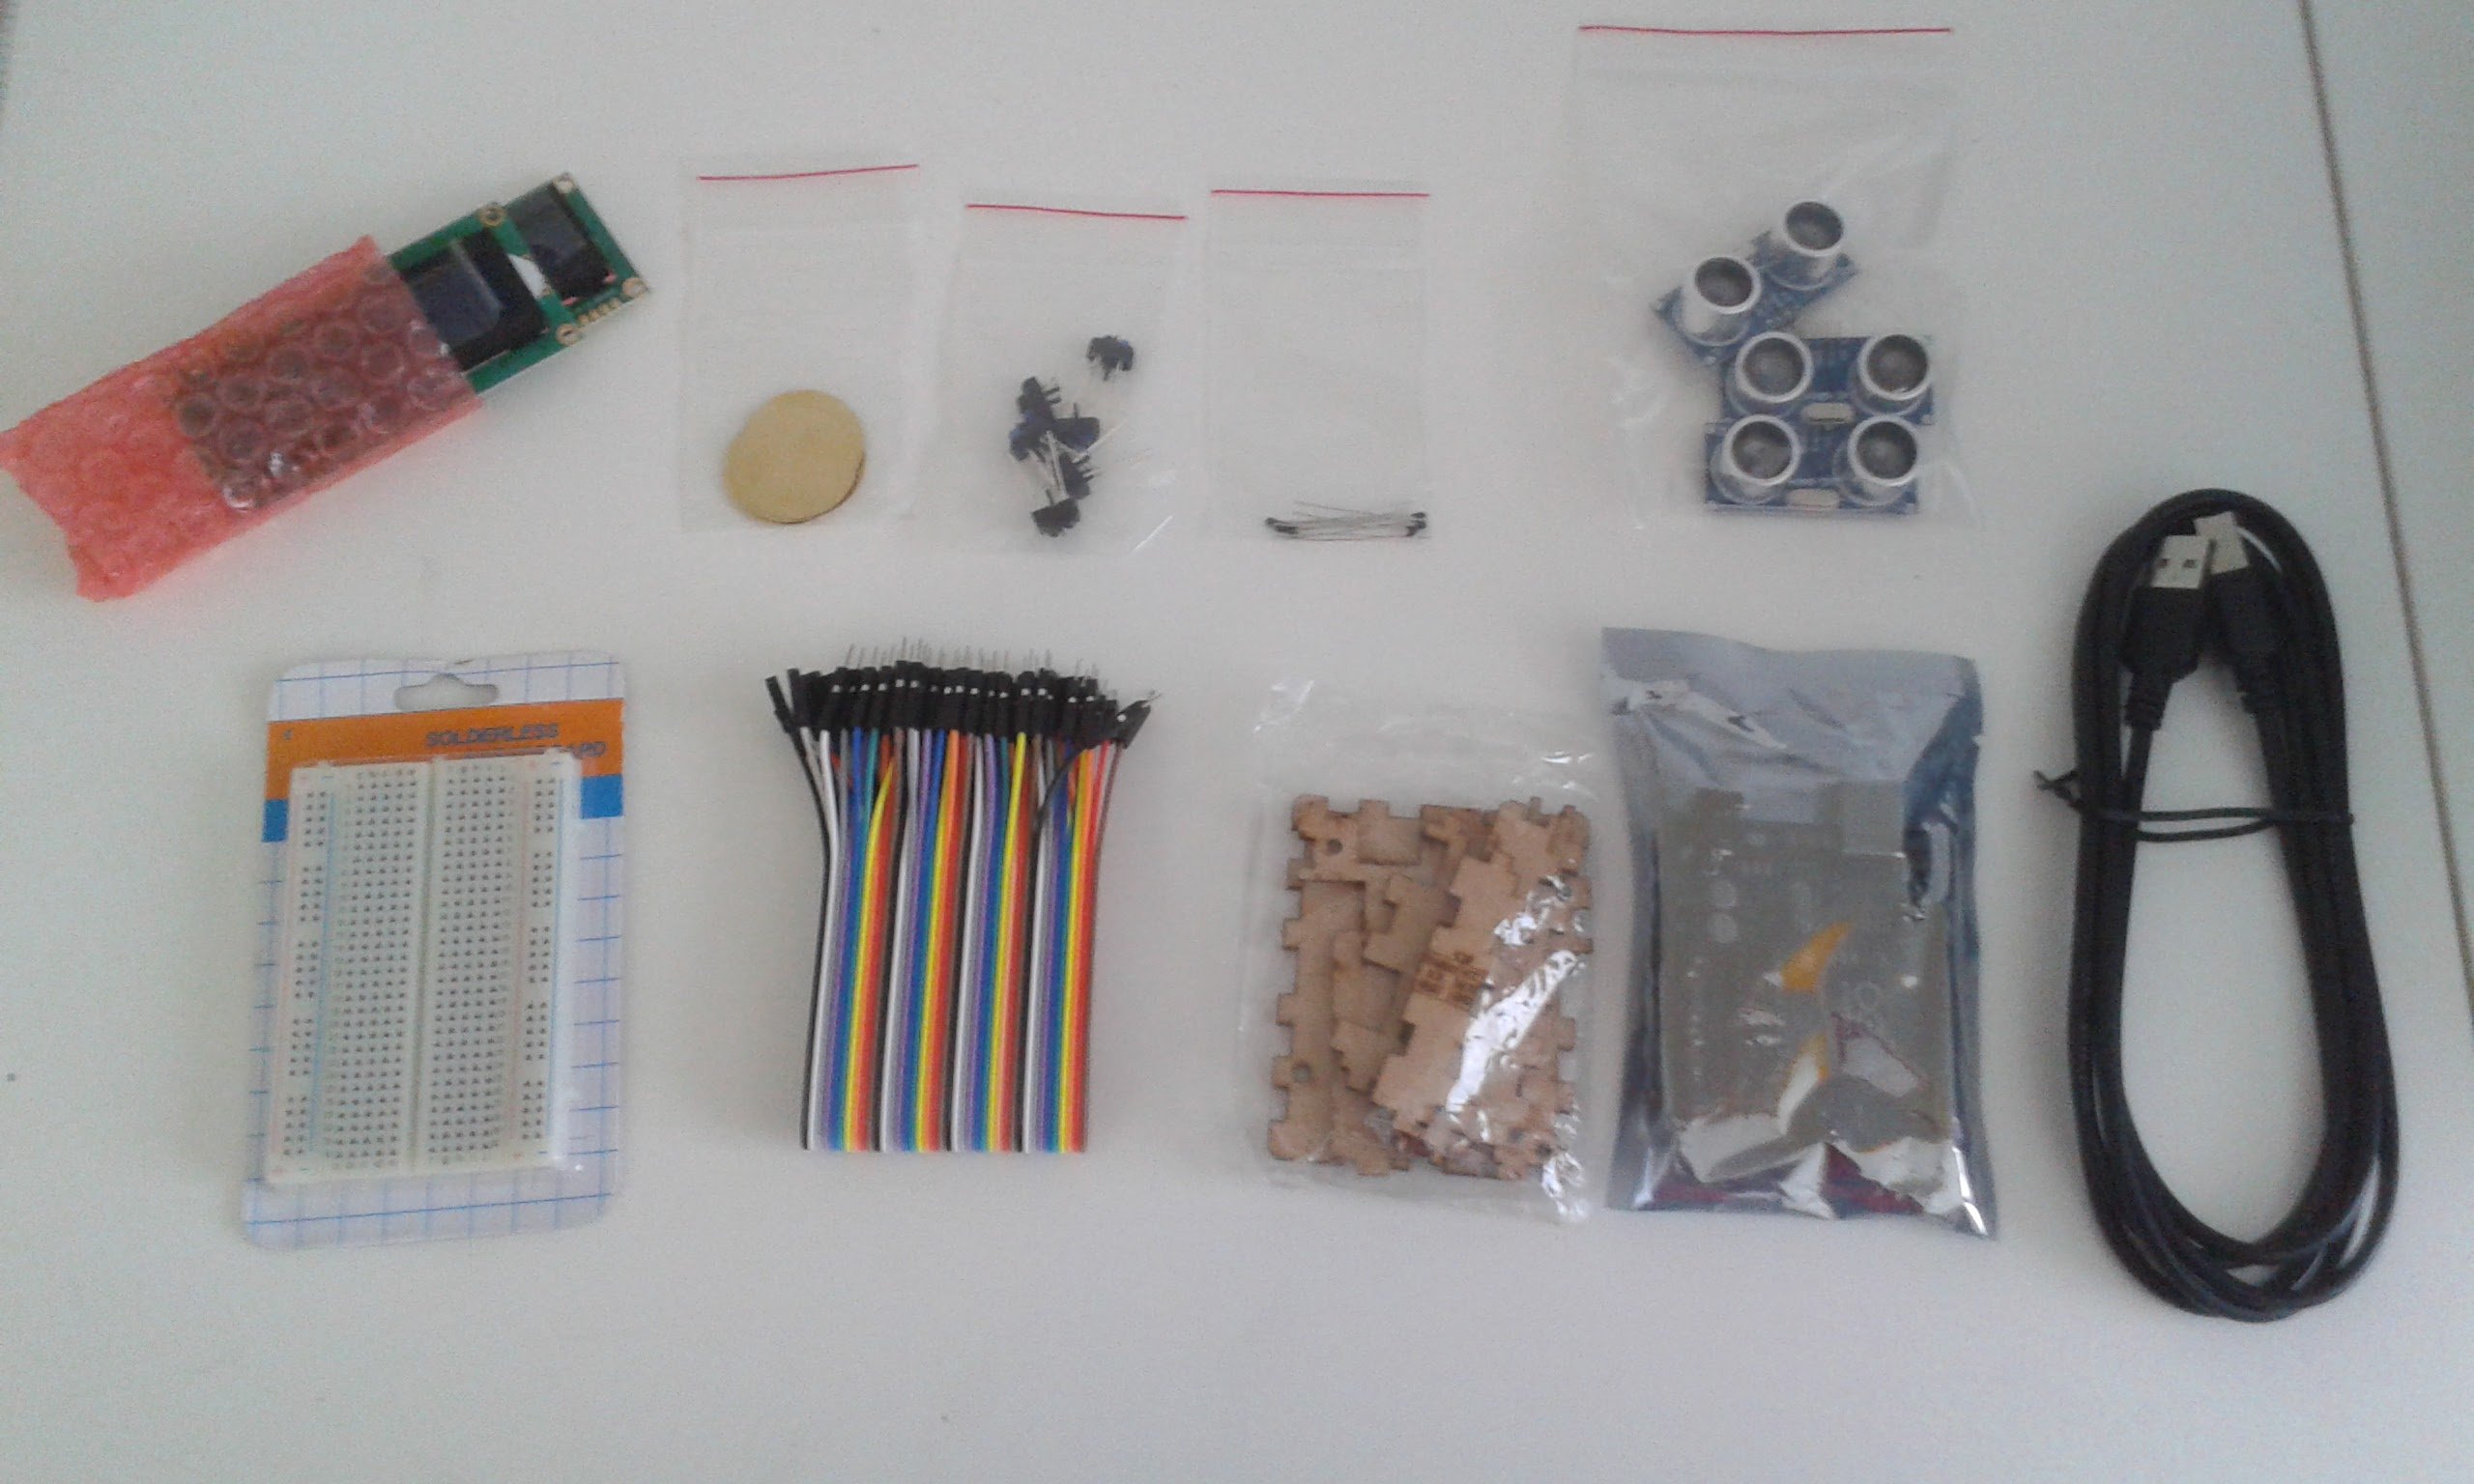
\includegraphics[width=0.8\linewidth]{materiais.jpg}
\caption{Materiais utilizados para aplicação com Arduino.}
\label{fig:materiais-arduino}
\end{figure}

%----------------------------------------------------------------------------------------
%	CONCLUSIONS
%----------------------------------------------------------------------------------------

\color{SaddleBrown} % SaddleBrown color for the conclusions to make them stand out

\section*{Conclusões}

\begin{itemize}
\item Os roteiros de prática precisam periodicamente passar por revisão técnica, bem como atualizações, buscando contextualizar os experimentos de físicas dentro do âmbito das engenharias.
\item A qualidade tipográfica dos roteiros das práticas deve ser vista como ponto importante, visto que um \emph{design} de baixa qualidade desmotiva a leitura e o aprendizado do conteúdo escrito.
\item O envolvimento de estudantes com o desenvolvimento de atividades que visam melhorar o curso possui um impacto positivo, estimulando os mesmos, assim como futuros alunos, à busca de excelência em suas atividades.
\end{itemize}

%----------------------------------------------------------------------------------------
%	FORTHCOMING RESEARCH
%----------------------------------------------------------------------------------------

\color{DarkSlateGray} % Set the color back to DarkSlateGray for the rest of the content

\section*{Próximos passos}

Pretendemos revisar ainda mais práticas de laboratório, aprimorando os roteiros e os próprios experimentos.
Pretendemos também padronizar os textos dos manuais de laboratório utilizando a linguagem de formatação \LaTeX.
Em alguns experimentos, pretendemos adaptar a plataforma \emph{Arduino} de forma a melhorar a precisão dos dados obtidos através de sensores.

 %----------------------------------------------------------------------------------------
%	REFERENCES
%----------------------------------------------------------------------------------------

%\nocite{*} % Print all references regardless of whether they were cited in the poster or not
%\bibliographystyle{plain} % Plain referencing style
%\bibliography{LabFisica} % Use the example bibliography file sample.bib

\printbibliography

%----------------------------------------------------------------------------------------
%	ACKNOWLEDGEMENTS
%----------------------------------------------------------------------------------------

\section*{Agradecimentos}

Gostaríamos de agradecer à Universidade de Fortaleza pelo apoio à este projeto, e disponibilidade dos laboratórios didáticos de Física, assim como aos professores e técnicos que nos auxiliam com discussões e suporte técnico relacionado aos equipamentos de laboratório.


%----------------------------------------------------------------------------------------

\end{multicols}
\end{document}